\documentclass[]{article}%{ctexart}
\pagestyle{empty}
\usepackage[table]{xcolor}
% QCC book needs
\usepackage{fix-cm}  % this package allows large \fontsize
\usepackage{imakeidx}
\makeindex[title=Index]
\usepackage{listings}
\usepackage[table]{xcolor}

\usepackage{amsmath,graphicx}

\usepackage{tikz}    % this is for graphics. e.g. rectangle on title 
\usetikzlibrary{quantikz, decorations.pathmorphing,shapes.geometric}
%\usepackage{circuitikz}
\usepackage{tikz-3dplot} % includes tikz
\tdplotsetmaincoords{70}{120}
\usepackage{float}


% This file is for commands / macros / functions.
% QCC book specific
\newcommand{\keta}[2][]{\vert {#2} \rangle_{#1}}
\newcommand{\braketa}[3][]{\langle {#2} \vert {#3}\rangle_{#1}}

\tikzstyle{Gate}=[rectangle, minimum width=30, minimum height=30, text width=20, text centered, draw=black]

\begin{document}

%\label{qQPSK}
\begin{tikzpicture}
    \draw[->] (-3.2,0) -- (3.5, 0);
    \draw[->] (0,-3.2) -- (0,3.5);
    \draw[gray, dashed] (2.4,2.4) -- (0,0);
    \draw[gray,dashed] (0,0) -- (2.3,-2.3);
    \draw[dotted, red] (0,0) circle(3cm);
    \draw[red, fill] (3,0) circle(0.05cm) node[below right] {$\keta{0}$ - 00};
    \draw[red, fill] (0,3) circle(0.05cm) node[above right] {$\keta{1}$ - 01};
    \draw[red, fill] (2.12,2.12) circle(0.05cm) node[right=0.3] {$\keta{+}$ - 11};
    \draw[red, fill] (2.12,-2.12) circle(0.05cm) node[below=0.5, right] {$\keta{-}$ - 10};
    \draw[dashed] (1,0) arc (0:45:1) node[right, pos=0.6]{$\theta=\pi/4$};
\end{tikzpicture}

%\label{8QAM}
\begin{tikzpicture}
    \draw[->] (-3.5,0) -- (3.5, 0);
    \draw[->] (0,-3.5) -- (0,3.5);
    \draw[gray, dashed] (2.5,2.5) -- (-2.5,-2.5);
    \draw[gray, dashed] (-2.5,2.5) -- (2.5,-2.5);
    \draw[dotted, red] (0,0) circle(2cm);
    \draw[dotted, red] (0,0) circle(3cm);
    \draw[red, fill] (270:2) circle(0.05cm) node[above left] {11};
    \draw[red, fill] (90:2) circle(0.05cm) node[above right] {01};
    \draw[red, fill] (0:2) circle(0.05cm) node[above left] {00};
    \draw[red, fill] (180:2) circle(0.05cm) node[above right] {10};
    \draw[red, fill] (45:3) circle(0.05cm) node[right] {111};
    \draw[red, fill] (135:3) circle(0.05cm) node[left] {101};
    \draw[red, fill] (225:3) circle(0.05cm) node[left] {100};
    \draw[red, fill] (-45:3) circle(0.05cm) node[right] {110};
\end{tikzpicture}

%\label{16QAM}
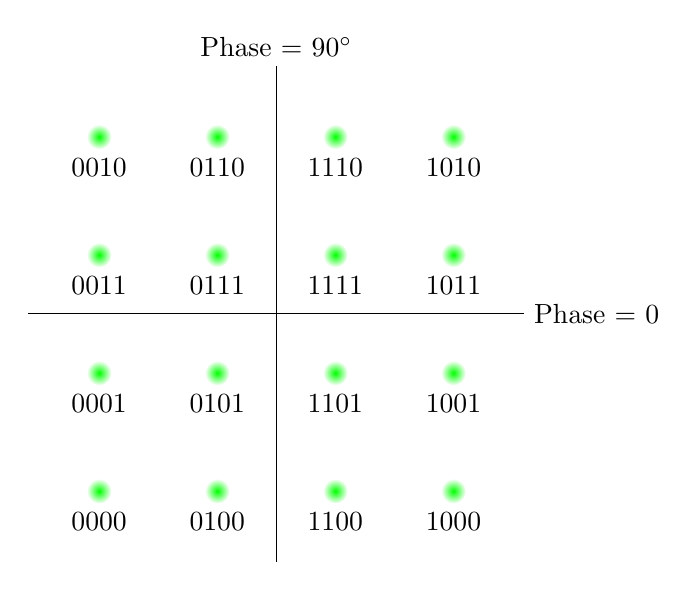
\begin{tikzpicture}[scale=1.5]

% Axis
\draw[] (-2.1,0) -- (2.1,0) node[right] {Phase = 0};
\draw[] (0,-2.1) -- (0,2.1) node[above] {Phase = $90^\circ$};

% Constellation points and labels
\foreach \x/\ix in {-1.5/00, -0.5/01, 0.5/11, 1.5/10} {
    \foreach \y/\iy in {-1.5/00, -0.5/01, 0.5/11, 1.5/10} {
        \shade[shading=radial, inner color=green, outer color=white]  (\x, \y) circle (3pt); % Larger circle with fading edge
        \node[anchor=north] at (\x, \y - 0.1) {\ix\iy}; % Shift labels slightly below
    }
}
\end{tikzpicture}

\end{document}